\chapter{Sandboxing 各种实现的分析与对比}
\label{s:evaluation}

\section{实现比较}
\label{ss: comparision}

\begin{figure}[!htp]
  \centering
  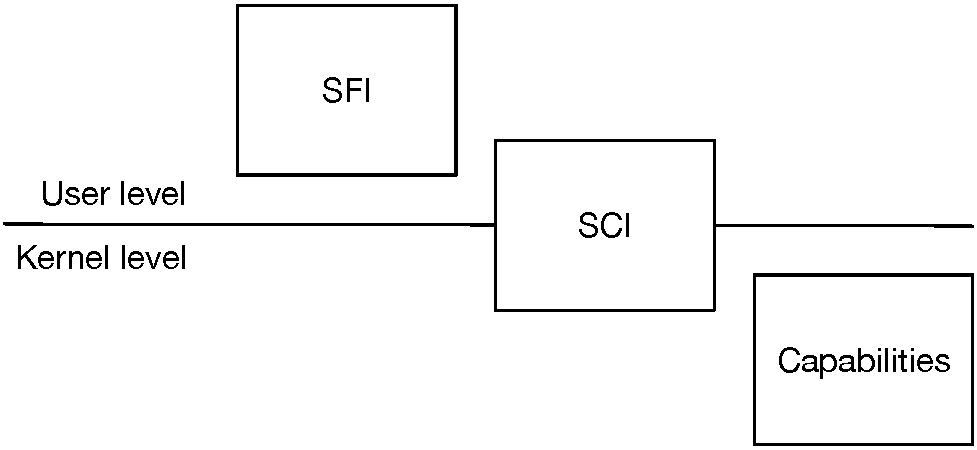
\includegraphics[width=0.7\linewidth]{imgs/difference}
  \caption{三种实现的比较}
  \label{fig:difference}
\end{figure}

在分类中,SFI 属于第一类沙箱,而 SCI 和 Capability 属于第二类沙箱。它们各自的实现如图 \ref{fig:difference} 所示,分别是实现在用户态,内核态以及在内核态和用户态都有一部分实现。其中 SFI 是完全用户态的实现,依靠二进制改写或修改编译器等等方式来进行错误的隔离。这样的实现相比于其他两种技术的实现方式,会更加简单。但是 SFI 的实现往往会依赖操作系统的 API 或者 ABI,这使得对于不同的处理器架构而言,要进行不同的实现,普适性不是很好。Native Client 最初是在 X86 架构上实现的。其后的论文 \parencite{sehr2010adapting} 介绍了 SFI 在 ARM 和 X86-64 架构上的实现方式。相比于 X86 的实现,就会有一些不同的实现思路。

而 SCI 要求在内核态和用户态都要进行一定的实现,因为 SCI 的 policy engine 往往是在用户态运行,而真正处理系统调用的逻辑是在内核中完成的。SCI 能够过滤所有不合法的系统调用,这是其主要关注的问题,也是其他两种方式实现不了的。但是 SCI 的缺点也是非常明显的:time-of-check/time-of-use 竞争问题 \parencite{bishop1996checking}。因为 SCI 在用户态检查合法性,而在内核态执行真正的系统调用,所以权限检查与系统调用的执行不是原子性的。这就带来了数据竞争的问题。在早期的 Janus 实现中,会出现全局、进程间和线程间三种数据竞争。而 Ostia 通过改变了实现的架构,解决了后两者的数据竞争的问题,对于前者,Ostia 采取了一种相对而言不太严谨的做法来规避了问题的发生,因为 Ostia 的 委托架构,使得 Agent 可以重新组织系统调用使得应用发起的系统调用遵循操作系统的惯例。但是我们认为这样有可能会导致一些对顺序敏感的应用程序在调用时产生顺序上的错误,并没有完全解决问题。

Capability其实严格来说是一种安全哲学,作为这三者中唯一可以完全植根于内核态的安全框架,其向用户暴露的主要是系统调用以及运行组件,最大的优势在于遵从POLP,做到了细粒度的AC,并维护了细粒度任务到细粒度权限的映射,从而避免了由于混淆所导致的confused deputies problem;同时,相较于传统的基于ACL的权限策略,更具灵活性。但是传统思路下实现的Capability存在明显的技术限制,且有较大的编程难度,所以很少在商用OS中得到推广。Capsicum作为被纳入FreeBSD9的一种基于Capability的安全框架,以其讨巧的设计在安全性与额外开销之间找到了一个可行的平衡点,但如何以更小的代价得到更高的安全性仍是需要不断探索的方向。

\section{性能分析}
\label{ss: analysis}

沙箱技术在提高了隔离性的同时,不可避免地为系统引入了新的 overhead。由于三者的实现不同,因此有着不同的 overhead。这三种沙箱技术的 overhead 大多体现在网络,计算和系统调用上。三者的研究论文并不是完全按照这三个不同子系统的 overhead 来进行验证与测试的,但是其测试结果从侧面反映出了在三者之上的性能损耗。

以 Janus、Ostia 为代表的 SCI 技术,关注过滤系统调用请求。因此该实现在网络和计算上的性能损耗非常小,基本可以忽略不计。Ostia 是在我们所见的论文中,唯一一个以这三方面作为不同的研究对象进行性能损耗的讨论的,Ostia 在对网络和计算的测量中,两者的 overhead 均没有超过 1\%,而在系统调用方面,改进后的 Janus \parencite{wagner1999janus} 有 8\% 的 overhead,而 Osita 因为委托架构的实现,在解决了部分数据竞争问题的同时,带来了 25\% 的 overhead。

SFI 相比于 SCI,性能损耗更多体现在计算上,而在网络和系统调用上都可以忽略不计。在计算方面,SFI 的 overhead 体现在:

\begin{itemize}
\item
使用 SFI 技术对 store 和 jmp 等指令进行保护检查。这是 SFI 性能损耗最大的一点,平均有 22\%。Native Client 对原本的实现有所改进,但是并没有质的改变,仍然是同一数量级。
\item
以及为了实现 SFI 向原本的二进制中插入的指令的长度。SFI 需要多余的指令完成检查的逻辑,因此支持 SFI 的二进制文件会比不支持 SFI 的文件多 10\% 左右的指令。
\item
相比于传统的执行多使用的寄存器数目。因为 SFI 使用了栈寄存器等,因此在寄存器数目上也存在 overhead,但这基本可以忽略不计。
\end{itemize}

综合来看,SFI 在计算上有平均 5\% 的 overhead。

以Capsicum为代表的基于capability的安全框架主要是在内核中实现,故其overhead主要可以通过三个维度来衡量:系统调用、沙盒创建,以及实际程序的执行。将相关测试结果用基于置信度为 95\%的T检验进行分析,可得:Capsicum所提供的API,相较于原生的UNIX POSIX的API,造成了大约 10\% 的overhead;而沙盒创建(即cap\_enter),达到了与chroot相似的overhead,而相较于fork,则造成了 9\% 的overhead;在实际程序的执行上,以gzip为例可见,capability所造成的overhead主要来自于诸如沙盒创建等初始阶段,所以当任务较为琐碎的时候(在gzip样例中表现为文件大小较小),capability会产生明显且非常稳定的overhead,而当任务变大时,capability版本的程序与原程序几乎没有表现出明显的性能差异。

综合来看,capability不可避免地会产生一定的overhead,且这些overhead主要来自于沙盒创建,及相关接口调用(如由fd生成相应的Capability)等,平均上有9\%左右的overhead,且能随着单个程序本身的业务逻辑的增大而得到均摊。

值得一提的是,Capsicum的作者尝试从另一个角度来看待这个问题 \parencite{capsicum}:任何安全隔离都不可避免地带来开销,换言之,任何security-critical的程序的设计者其实都默认接受了一定的overhead,所以不如以“如何用一定的overhead来换取更好的安全性”作为问题的核心。虽然这一点就测试而言,似乎该怎么测试还得怎么测试,但是我们认为,在系统设计之初就抱有这样的想法的话,不失为另辟蹊径的一种策略,可作参考。
